% =====================================================================
%  RobustLeaf-Net : IEEE conference-format paper (IEEEtran)
%  Compile on Overleaf (pdfLaTeX) or locally:  pdflatex main.tex (x2)
%
%  Anything printed in RED is still a placeholder. After the experiments run:
%     python fill_paper.py ...          (writes numbers.tex + results_rows.tex)
%     python make_paper_figures.py ...  (writes figs/*.png)
%  then recompile: values and figures appear automatically and the red
%  placeholders disappear. Author names/affiliations/acknowledgment are
%  the only red items you must type yourself.
% =====================================================================
\documentclass[conference]{IEEEtran}
\IEEEoverridecommandlockouts

\usepackage{cite}
\usepackage{amsmath,amssymb,amsfonts}
\usepackage{algorithmic}
\usepackage{graphicx}
\usepackage{textcomp}
\usepackage{xcolor}
\usepackage{booktabs}
\usepackage{array}
\usepackage{tikz}
\usetikzlibrary{arrows.meta,positioning,calc}
\def\BibTeX{{\rm B\kern-.05em{\sc i\kern-.025em b}\kern-.08em
    T\kern-.1667em\lower.7ex\hbox{E}\kern-.125emX}}

% red placeholder for values that still have to be filled in
\newcommand{\tbd}[1]{\textcolor{red}{#1}}
% ---- values filled automatically by fill_paper.py (numbers.tex) ----
\newcommand{\AccIn}{\tbd{XX.X}}\newcommand{\AccField}{\tbd{XX.X}}
\newcommand{\AccFieldBase}{\tbd{XX.X}}\newcommand{\SizeMB}{\tbd{XX}}
\newcommand{\ParamsM}{\tbd{X.X}}\newcommand{\LatencyMs}{\tbd{XX}}
\newcommand{\FieldN}{\tbd{N}}\newcommand{\FieldM}{\tbd{M}}
\newcommand{\GPUName}{\tbd{[GPU model]}}\newcommand{\DeviceName}{\tbd{[CPU/GPU model]}}
\newcommand{\dInA}{\tbd{$\pm$X.X}}\newcommand{\dFieldA}{\tbd{$\pm$X.X}}
\newcommand{\dFieldB}{\tbd{$\pm$X.X}}\newcommand{\gapB}{\tbd{XX.X}}
\newcommand{\gapC}{\tbd{XX.X}}\newcommand{\dFieldC}{\tbd{$\pm$X.X}}
\newcommand{\dFieldD}{\tbd{$\pm$X.X}}
\newcommand{\AutoDiscussion}{\tbd{[Generated by fill\_paper.py from the measured results.]}}
\newcommand{\FocusA}{\tbd{XX.X}}\newcommand{\FocusB}{\tbd{XX.X}}
\newcommand{\ResultsRows}{%
 \tbd{A0} & \tbd{XX.X} & \tbd{XX.X} & \tbd{XX.X} & \tbd{XX.X} & \tbd{X.XX} & \tbd{XX.X} & \tbd{XX.X} \\
 \tbd{A1} & \tbd{XX.X} & \tbd{XX.X} & \tbd{XX.X} & \tbd{XX.X} & \tbd{X.XX} & \tbd{XX.X} & \tbd{XX.X} \\
 \tbd{A2} & \tbd{XX.X} & \tbd{XX.X} & \tbd{XX.X} & \tbd{XX.X} & \tbd{X.XX} & \tbd{XX.X} & \tbd{XX.X} \\
 \tbd{A3} & \tbd{XX.X} & \tbd{XX.X} & \tbd{XX.X} & \tbd{XX.X} & \tbd{X.XX} & \tbd{XX.X} & \tbd{XX.X} \\
 \tbd{A4} & \tbd{XX.X} & \tbd{XX.X} & \tbd{XX.X} & \tbd{XX.X} & \tbd{X.XX} & \tbd{XX.X} & \tbd{XX.X} \\
 \tbd{A5} & \tbd{XX.X} & \tbd{XX.X} & \tbd{XX.X} & \tbd{XX.X} & \tbd{X.XX} & \tbd{XX.X} & \tbd{XX.X} \\}
\IfFileExists{numbers.tex}{\input{numbers.tex}}{}
\IfFileExists{results_rows.tex}{\input{results_rows.tex}}{}
% figure from file if it exists, otherwise a red placeholder box
\newcommand{\figorbox}[3]{\IfFileExists{#1}{\includegraphics[width=#2]{#1}}{\fbox{\parbox{#2}{\centering\vspace{14mm}\tbd{#3}\vspace{14mm}}}}}

\begin{document}

\title{RobustLeaf-Net: Closing the Lab-to-Field Gap in Plant Disease Recognition with Background Randomization and Mask-Guided Attention}

\author{
\IEEEauthorblockN{Tejas Wadekar, Vishwesh Kalled, Shrishant Mugalikar, and Vedant Balekundri}
\IEEEauthorblockA{\textit{Anuvartik Mirji Bharatesh Institute of Technology}\\
Belgaum, Karnataka, India\\
vpp22cstejassw@gmail.com, kalledvishwesh@gmail.com,\\
shrishantmugalikar313@gmail.com, vedantbalekundrii@gmail.com}
}

\maketitle

\begin{abstract}
Deep learning models reach near-perfect accuracy on the PlantVillage benchmark, yet their accuracy often falls on photographs taken in the field. A likely cause is that laboratory images have clean, uniform backgrounds, which lets networks learn background shortcuts instead of disease symptoms. This paper presents RobustLeaf-Net, a lightweight transfer-learning framework that targets this lab-to-field gap with three components: (i)~Saturation-based Background Randomization (SBR), an augmentation that estimates the leaf region from colour saturation and replaces the background with random colour and noise; (ii)~Mask-Guided Attention (MGA), in which the spatial attention map of a CBAM block is supervised by the same automatically estimated leaf mask, so no manual annotation is needed; and (iii)~hierarchical crop and disease heads with crop-consistent decoding. The model is built on MobileNetV2 and is complemented by Grad-CAM explanations, a colour-based severity estimate and an automatically generated PDF disease report served through a web application. We evaluate the method with a six-step ablation (A0--A5) on PlantVillage and on held-out field images. The full model reaches \AccIn\% accuracy on PlantVillage and \AccField\% on field images, compared with \AccFieldBase\% on field images for the plain transfer-learning baseline, with a model size of \SizeMB~MB.
\end{abstract}

\begin{IEEEkeywords}
plant disease detection, deep learning, transfer learning, attention mechanism, domain generalization, Grad-CAM, precision agriculture
\end{IEEEkeywords}

%======================================================================
\section{Introduction}
Plant diseases reduce crop yield and quality and are a major threat to food security, particularly for smallholder farmers who rarely have quick access to plant pathologists. Image-based diagnosis with convolutional neural networks (CNNs) offers a low-cost alternative, and the public PlantVillage dataset~\cite{hughes2015} has made it possible to train classifiers that exceed 95\% accuracy on its test split~\cite{mohanty2016,ferentinos2018}.

However, high benchmark accuracy does not guarantee reliable field performance. Barbedo~\cite{barbedo2018} reports that dataset size, symptom variability and image-capture conditions strongly affect how well deep models generalize. PlantVillage images are taken on a uniform background under controlled light, so a network can partly rely on background and capture-condition cues rather than on the lesion itself. This behaviour is an example of shortcut learning~\cite{geirhos2020}, and it is known that image backgrounds can carry class-correlated signal that models exploit~\cite{xiao2021}. The consequence is a \emph{lab-to-field gap}: accuracy measured on laboratory images overstates accuracy on real farm photographs.

This work addresses that gap with an inexpensive, annotation-free approach. Our contributions are:
\begin{itemize}
\item \textbf{Saturation-based Background Randomization (SBR).} A training-time augmentation that estimates the leaf region from colour saturation and replaces the background with random colour and noise, removing the background shortcut.
\item \textbf{Mask-Guided Attention (MGA).} A loss that trains the spatial attention map of a CBAM block~\cite{woo2018} to match the automatically estimated leaf mask, steering the network towards the leaf without manual labels.
\item \textbf{Hierarchical heads with crop-consistent decoding.} Joint crop and disease prediction in which only diseases of the predicted crop are allowed at inference.
\item \textbf{Complete diagnosis pipeline.} Grad-CAM explanations, a colour-based severity estimate, a disease knowledge base and an automatic PDF report, delivered through a web application.
\item \textbf{Evaluation protocol.} A six-step ablation with in-domain and cross-domain tests, a generalization-gap metric and efficiency measurements, repeated over three random seeds.
\end{itemize}

The remainder of the paper is organized as follows. Section~II reviews related work, Section~III describes the method, Section~IV the experimental setup, Section~V the results, Section~VI the deployed system, and Section~VII concludes.

%======================================================================
\section{Related Work}
\subsection{Deep Learning for Plant Disease Recognition}
Mohanty et al.~\cite{mohanty2016} trained AlexNet and GoogLeNet on PlantVillage and reported accuracy above 99\% on random splits, while also observing a large drop when models were tested on images from other conditions. Ferentinos~\cite{ferentinos2018} compared several architectures, including VGG~\cite{simonyan2015} and others, on a larger open image database. Later work has relied on transfer learning from ImageNet~\cite{deng2009} with ResNet~\cite{he2016}, MobileNetV2~\cite{sandler2018} and EfficientNet~\cite{tan2019}. The PlantDoc dataset~\cite{singh2020} was introduced precisely because models trained on laboratory data transfer poorly to images with natural backgrounds.

\subsection{Shortcut Learning and Background Bias}
Geirhos et al.~\cite{geirhos2020} describe how networks adopt decision rules that work on a benchmark but fail under distribution shift. Xiao et al.~\cite{xiao2021} study the role of image backgrounds in object recognition and show that models can exploit them. These findings motivate our background randomization, which is a targeted form of data augmentation~\cite{shorten2019} designed to break the link between background and label.

\subsection{Attention and Lightweight Backbones}
The Convolutional Block Attention Module (CBAM)~\cite{woo2018} refines features with sequential channel and spatial attention and adds few parameters. Lightweight backbones such as MobileNetV2~\cite{sandler2018} make on-device or low-cost deployment feasible. We combine both, and, unlike standard CBAM, we supervise the spatial attention with an automatically derived leaf mask.

\subsection{Explainability}
Grad-CAM~\cite{selvaraju2017} produces class-discriminative heat maps from gradients of the class score with respect to the last convolutional feature maps. We use it to show whether the model attends to the leaf and lesions instead of the surroundings.

%======================================================================
\section{Proposed Method}
\subsection{Overview}
Fig.~\ref{fig:arch} shows RobustLeaf-Net. An input leaf image of size $224\times224$ passes through the SBR augmentation (training only), a pre-trained MobileNetV2 backbone~\cite{sandler2018}, a CBAM block, global average pooling and dropout. Three heads follow: a disease classifier, a crop classifier, and the spatial attention map that is trained against the estimated leaf mask.

\begin{figure*}[!t]
\centering
\resizebox{0.97\textwidth}{!}{%
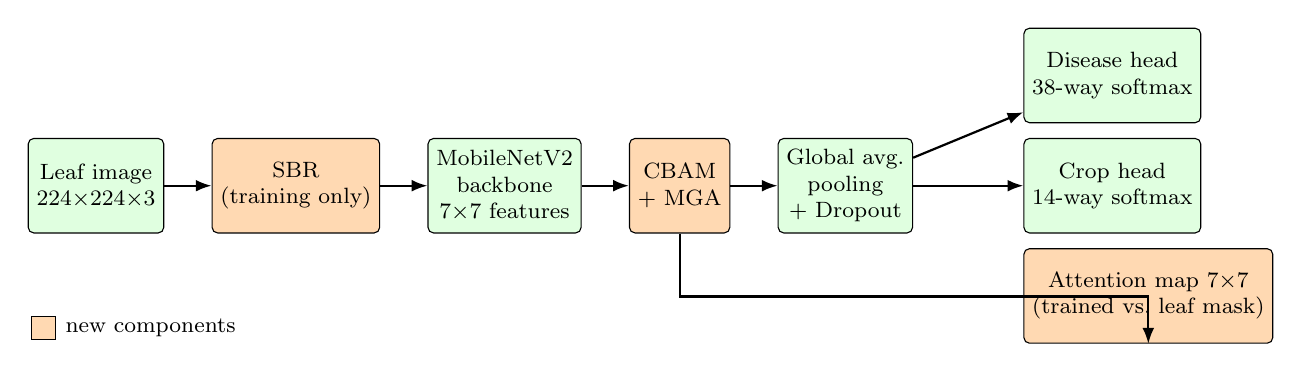
\begin{tikzpicture}[node distance=6mm,
  blk/.style={draw, rounded corners=2pt, minimum height=12mm, align=center, fill=green!12, inner sep=3pt, font=\footnotesize},
  new/.style={blk, fill=orange!30},
  arr/.style={-{Latex[length=2mm]}, thick}]
\node[blk] (in) {Leaf image\\$224{\times}224{\times}3$};
\node[new, right=of in] (sbr) {SBR\\(training only)};
\node[blk, right=of sbr] (bb) {MobileNetV2\\backbone\\$7{\times}7$ features};
\node[new, right=of bb] (cbam) {CBAM\\+ MGA};
\node[blk, right=of cbam] (gap) {Global avg.\\pooling\\+ Dropout};
\node[blk, right=14mm of gap, yshift=14mm] (h1) {Disease head\\38-way softmax};
\node[blk, right=14mm of gap] (h2) {Crop head\\14-way softmax};
\node[new, right=14mm of gap, yshift=-14mm] (h3) {Attention map $7{\times}7$\\(trained vs.\ leaf mask)};
\draw[arr] (in)--(sbr);
\draw[arr] (sbr)--(bb);
\draw[arr] (bb)--(cbam);
\draw[arr] (cbam)--(gap);
\draw[arr] (gap)--(h1);
\draw[arr] (gap)--(h2);
\draw[arr] (cbam.south) -- ++(0,-8mm) -| (h3.south);
\node[draw, fill=orange!30, minimum size=3mm, label=right:{\footnotesize new components}] at ($(in.south west)+(2mm,-12mm)$) {};
\end{tikzpicture}}
\caption{Architecture of RobustLeaf-Net. Orange blocks are the proposed components: background randomization (SBR) applied to training images, and the CBAM spatial attention map supervised by the estimated leaf mask (MGA). At test time the disease and crop outputs give the diagnosis.}
\label{fig:arch}
\end{figure*}

\subsection{Leaf-Mask Estimation}
Laboratory backgrounds are grey, white or black and therefore have low colour saturation, whereas healthy and diseased leaf tissue (green, yellow, brown) is more saturated. For an RGB image $x$ we convert to HSV, threshold the saturation channel $S(x)$, and apply a morphological closing (dilation followed by erosion with a $5\times5$ window):
\begin{equation}
M = \mathrm{Close}\big(\mathbb{1}[\,S(x) > \tau\,]\big),\qquad \tau = 0.15 .
\label{eq:mask}
\end{equation}
No manual segmentation is required.

\subsection{Saturation-based Background Randomization (SBR)}
During training, with probability $p=0.5$ per image, the background is replaced by a random colour with additive Gaussian noise:
\begin{equation}
\tilde{x} = \tilde{M}\odot x + (1-\tilde{M})\odot b,\quad b=\mathrm{clip}\big(c\mathbf{1}+\epsilon\big),
\label{eq:sbr}
\end{equation}
where $c\sim\mathcal{U}(0,255)^3$, $\epsilon\sim\mathcal{N}(0,\sigma^2)$ with $\sigma=25$, and $\tilde{M}$ is $M$ smoothed with a $5\times5$ mean filter to avoid hard cut-out edges. The mask is passed through the same geometric augmentations as the image so that both remain aligned.

\begin{figure*}[!t]
\centering
\resizebox{0.95\textwidth}{!}{%
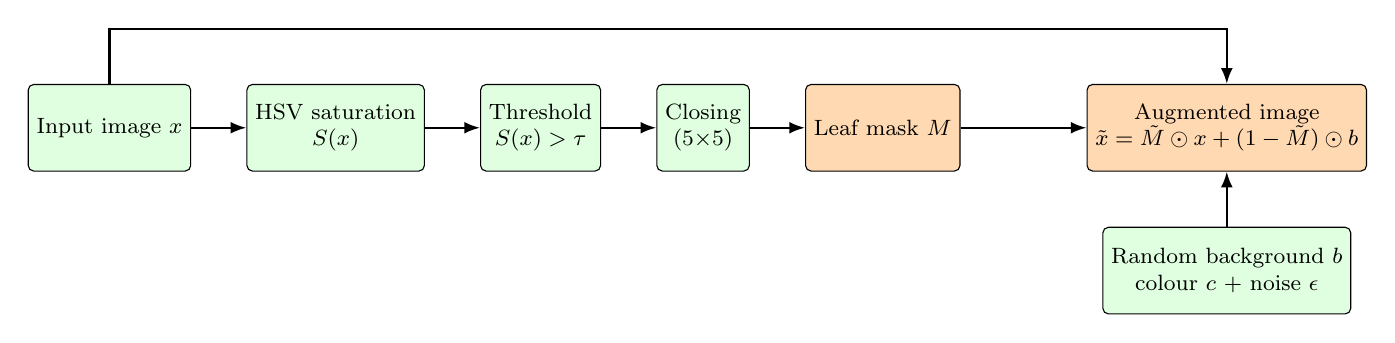
\begin{tikzpicture}[node distance=7mm,
  blk/.style={draw, rounded corners=2pt, minimum height=11mm, align=center, fill=green!12, inner sep=3pt, font=\footnotesize},
  new/.style={blk, fill=orange!30},
  arr/.style={-{Latex[length=2mm]}, thick}]
\node[blk] (x) {Input image $x$};
\node[blk, right=of x] (hsv) {HSV saturation\\$S(x)$};
\node[blk, right=of hsv] (thr) {Threshold\\$S(x)>\tau$};
\node[blk, right=of thr] (cl) {Closing\\($5{\times}5$)};
\node[new, right=of cl] (m) {Leaf mask $M$};
\node[new, right=16mm of m] (out) {Augmented image\\$\tilde{x}=\tilde{M}\odot x+(1-\tilde{M})\odot b$};
\node[blk, below=7mm of out] (b) {Random background $b$\\colour $c$ + noise $\epsilon$};
\draw[arr] (x)--(hsv); \draw[arr] (hsv)--(thr); \draw[arr] (thr)--(cl); \draw[arr] (cl)--(m);
\draw[arr] (m)--(out); \draw[arr] (b)--(out);
\draw[arr] (x.north) -- ++(0,7mm) -| (out.north);
\end{tikzpicture}}
\caption{Saturation-based Background Randomization (SBR). The leaf mask is estimated from colour saturation without manual labels; the background is then replaced by a random colour with noise (applied to each training image with probability $p=0.5$).}
\label{fig:sbr}
\end{figure*}

\begin{figure}[!t]
\centering
\figorbox{figs/fig_sbr_examples.png}{\columnwidth}{Insert SBR examples (figs/fig\_sbr\_examples.png)}
\caption{Examples from PlantVillage: original image, estimated leaf mask, and two random SBR variants.}
\label{fig:sbr_examples}
\end{figure}

\subsection{CBAM with Mask-Guided Attention}
Let $F\in\mathbb{R}^{7\times7\times C}$ be the backbone feature map. CBAM~\cite{woo2018} applies channel attention $A_c$ and then spatial attention $A_s$:
\begin{equation}
F' = A_c(F)\otimes F,\qquad F'' = A_s(F')\otimes F',
\end{equation}
\begin{equation}
A_s(F') = \sigma\Big(f^{7\times7}\big([\mathrm{AvgPool}_c(F');\mathrm{MaxPool}_c(F')]\big)\Big),
\end{equation}
where the channel reduction ratio is 16. In MGA, the spatial map $A_s\in[0,1]^{7\times7}$ is additionally trained to match the leaf mask $M$ down-sampled to $7\times7$ by area interpolation ($M\!\downarrow$):
\begin{equation}
\mathcal{L}_{\mathrm{attn}} = -\frac{1}{HW}\sum_{i,j}\Big[m_{ij}\log a_{ij} + (1-m_{ij})\log(1-a_{ij})\Big],
\end{equation}
with $m=M\!\downarrow$ and $a=A_s$. The supervision is used only during training.

\subsection{Hierarchical Heads and Crop-Consistent Decoding}
The disease head predicts one of $K=38$ classes and the crop head one of 14 crops. Because every disease class belongs to exactly one crop, we define $\mathrm{crop}(k)$ and, at inference, restrict the disease prediction to the predicted crop $\hat{c}$:
\begin{equation}
\hat{y} = \arg\max_{k:\ \mathrm{crop}(k)=\hat{c}}\ p_k .
\label{eq:hier}
\end{equation}
This removes physically impossible predictions such as a tomato disease on a potato leaf.

\subsection{Training Objective and Procedure}
The total loss combines categorical cross-entropy terms for disease and crop with the attention loss:
\begin{equation}
\mathcal{L} = \mathcal{L}_{\mathrm{dis}} + \lambda_c\,\mathcal{L}_{\mathrm{crop}} + \lambda_a\,\mathcal{L}_{\mathrm{attn}},\qquad \lambda_c=0.3,\ \lambda_a=0.2 .
\label{eq:loss}
\end{equation}
Training has two stages. In stage~1 the ImageNet-pretrained backbone is frozen and only the new layers are trained (learning rate $10^{-3}$). In stage~2 the last 40 backbone layers are unfrozen and fine-tuned with learning rate $10^{-5}$; batch-normalization layers stay frozen for stability. We use Adam~\cite{kingma2015}, early stopping on validation loss and learning-rate reduction on plateau.

\subsection{Explanation, Severity Estimate and Report}
For a predicted class $c$, Grad-CAM~\cite{selvaraju2017} computes
\begin{equation}
L^{c}_{\mathrm{Grad\text{-}CAM}} = \mathrm{ReLU}\Big(\sum_k \alpha^c_k A^k\Big),\quad \alpha^c_k=\frac{1}{Z}\sum_{i,j}\frac{\partial y^c}{\partial A^k_{ij}},
\end{equation}
where $A^k$ are the feature maps of the backbone's last convolutional layer. For severity, lesion pixels are leaf pixels (Eq.~\ref{eq:mask}) that are not green, with green defined as $G>1.05R$ and $G>B$. The affected-area fraction is $s=|\text{lesion}|/|\text{leaf}|$, mapped to \emph{mild} ($s<10\%$), \emph{moderate} ($10\%\le s<30\%$) or \emph{severe} ($s\ge30\%$). This is an indicative colour-based estimate and not a laboratory measurement. A knowledge base covering all 38 classes supplies cause, symptoms, treatment and prevention, and a PDF report combines these with the diagnosis, confidence, top-3 predictions and the Grad-CAM image.

%======================================================================
\section{Experimental Setup}
\subsection{Datasets}
\textbf{In-domain.} We use the colour images of PlantVillage~\cite{hughes2015}: approximately 54{,}000 leaf images in 38 classes covering 14 crops. A stratified 70/15/15 train/validation/test split is created once with a fixed seed and reused by all experiments.

\textbf{Cross-domain (field).} To measure the lab-to-field gap, models trained on PlantVillage are tested on field images whose classes overlap with PlantVillage, taken from PlantDoc~\cite{singh2020} and/or images collected by the authors. The field set contains \FieldN{} images in \FieldM{} shared classes. Field images are never used for training or model selection.

\subsection{Compared Variants (Ablation)}
Table~\ref{tab:ablation_def} lists the six variants. Each adds one component to the previous variant, so the effect of every component can be isolated.

\begin{table}[!t]
\caption{Ablation variants}
\label{tab:ablation_def}
\centering
\small
\begin{tabular}{@{}ll@{}}
\toprule
Run & Configuration \\
\midrule
A0 & Baseline CNN trained from scratch \\
A1 & MobileNetV2 transfer learning \\
A2 & A1 + CBAM \\
A3 & A2 + Background Randomization (SBR) \\
A4 & A3 + Mask-Guided Attention (MGA) \\
A5 & A4 + hierarchical heads (full RobustLeaf-Net) \\
\bottomrule
\end{tabular}
\end{table}

\subsection{Implementation Details}
Images are resized to $224\times224$. Training augmentation uses horizontal and vertical flips, rotation up to $\pm36^\circ$, zoom up to 15\%, and random per-image brightness gain in $[0.8,1.2]$ and bias in $[-20,20]$; SBR is added in A3--A5. The baseline CNN has four blocks of $3\times3$ convolution, batch normalization, ReLU and max-pooling (32, 64, 128 and 256 filters), followed by global average pooling, dropout (0.4), a 256-unit dense layer, dropout (0.3) and a softmax layer. Transfer models use a dropout of 0.3 before the heads. Batch size is 32; stage~1 runs for at most 8 epochs and stage~2 for at most 12. Experiments are run with seeds 42, 1 and 2 and reported as mean $\pm$ standard deviation. The code is implemented in Python with TensorFlow/Keras~\cite{abadi2016}; training was done on \GPUName{}.

\subsection{Evaluation Metrics}
We report accuracy and macro-averaged precision, recall and F1 on the in-domain test split and on the field set. The generalization gap is
\begin{equation}
\Delta = \mathrm{Acc}_{\mathrm{in}} - \mathrm{Acc}_{\mathrm{field}} .
\end{equation}
To quantify where the model looks, we define a Grad-CAM \emph{leaf-focus score}, the share of the (normalized) Grad-CAM mass that lies inside the estimated leaf mask $M$:
\begin{equation}
\mathrm{LF} = \frac{\sum_{i,j} L^{c}_{ij}\,M_{ij}}{\sum_{i,j} L^{c}_{ij}},
\end{equation}
averaged over the field images. Efficiency is measured by parameter count, saved model size (MB) and inference latency per image (ms, batch size 1) on \DeviceName{}.

%======================================================================
\section{Results and Discussion}
% (values below are generated by fill_paper.py from runs/*/metrics.json)
\subsection{Ablation Study}
Table~\ref{tab:results} reports the results of A0--A5 and Fig.~\ref{fig:ablation} visualizes them. Relative to the scratch CNN (A0), the transfer-learning baseline (A1) changes in-domain accuracy by \dInA{} points and field accuracy by \dFieldA{} points. Adding CBAM (A2) changes field accuracy by \dFieldB{} points. Background randomization (A3) changes the generalization gap $\Delta$ from \gapB{} to \gapC{} points. Mask-guided attention (A4) and hierarchical heads (A5) change field accuracy by a further \dFieldC{} and \dFieldD{} points, respectively. The full model (A5) reaches \AccIn\% in-domain and \AccField\% on field images.

\begin{table*}[!t]
\caption{Ablation results (mean $\pm$ std over three seeds). Acc = accuracy, F1 = macro-F1, $\Delta$ = in-domain minus field accuracy. A5 is reported with crop-consistent decoding (Eq.~\ref{eq:hier}).}
\label{tab:results}
\centering
\small
\begin{tabular}{@{}lccccccc@{}}
\toprule
Run & In-domain Acc (\%) & In-domain F1 (\%) & Field Acc (\%) & $\Delta$ (pts) & Params (M) & Size (MB) & Latency (ms) \\
\midrule
\ResultsRows
\bottomrule
\end{tabular}
\end{table*}

\begin{figure}[!t]
\centering
\figorbox{figs/fig_ablation.png}{\columnwidth}{Insert ablation chart (figs/fig\_ablation.png)}
\caption{In-domain and field accuracy for variants A0--A5 (mean $\pm$ std over three seeds).}
\label{fig:ablation}
\end{figure}

\subsection{Per-class Behaviour}
Fig.~\ref{fig:cm} shows the confusion matrix of the full model on the PlantVillage test split. Per-class precision, recall and F1 are given in the accompanying classification report. By construction, crop-consistent decoding (Eq.~\ref{eq:hier}) removes errors across crops, so remaining errors are confusions between diseases of the same crop.

\begin{figure}[!t]
\centering
\figorbox{figs/fig_confusion.png}{0.95\columnwidth}{Insert confusion matrix (figs/fig\_confusion.png)}
\caption{Confusion matrix of RobustLeaf-Net (A5) on the PlantVillage test split.}
\label{fig:cm}
\end{figure}

\subsection{Qualitative Analysis with Grad-CAM}
Fig.~\ref{fig:gradcam} compares Grad-CAM maps of the transfer baseline (A1) and the full model (A5) on field images. We examine whether the highlighted region lies on the leaf and on lesions rather than on soil, hands or other background, and report the leaf-focus score LF: \FocusA\% for A1 and \FocusB\% for A5.

\begin{figure}[!t]
\centering
\figorbox{figs/fig_gradcam.png}{\columnwidth}{Insert Grad-CAM comparison (figs/fig\_gradcam.png)}
\caption{Grad-CAM heat maps on field images for the baseline (A1) and the proposed model (A5).}
\label{fig:gradcam}
\end{figure}

\subsection{Efficiency}
The full model has \ParamsM\,M parameters, a saved size of \SizeMB\,MB and a latency of \LatencyMs\,ms per image on \DeviceName{}, as reported in Table~\ref{tab:results}.

\subsection{Summary of Findings}
\AutoDiscussion

\subsection{Limitations}
The leaf mask is a colour heuristic: it can fail for low-saturation leaves, white or very bright backgrounds, strong shadows, or images with several leaves, and in these cases SBR and MGA receive an imperfect mask. The severity estimate is based on colour and is therefore only indicative. The field set is limited in size and class coverage, so the reported field accuracy applies to the shared classes only. The system also assumes a single leaf in the image and cannot detect that a photo does not show a plant. Finally, the treatment advice in the knowledge base is general guidance and must be checked against product labels and local recommendations.

%======================================================================
\section{System Implementation}
The trained model is wrapped in a Streamlit web application. A user uploads or captures a leaf photo and receives the crop, disease, confidence, estimated severity, top-3 predictions, the Grad-CAM image, and the cause, symptoms, treatment and prevention from the knowledge base. Predictions with confidence below 0.60 are flagged as uncertain and the user is asked to retake the photo. A one-page PDF disease report can be downloaded, and a command-line tool processes folders of field images in batch. The application can be deployed on a free hosting service or in a container.

%======================================================================
\section{Conclusion and Future Work}
We presented RobustLeaf-Net, a lightweight plant disease recognition framework that combines background randomization, mask-guided attention and hierarchical decoding to reduce the dependence on laboratory backgrounds, together with a Grad-CAM explanation module and an automatic disease report. The ablation protocol isolates the contribution of each component and measures the lab-to-field gap directly. On the field set the full model attains \AccField\% accuracy versus \AccFieldBase\% for the transfer-learning baseline, at \AccIn\% in-domain accuracy and a size of \SizeMB\,MB. Future work includes learning the leaf mask instead of using a colour heuristic, collecting a larger multi-crop field dataset, lesion segmentation for more reliable severity grading, and converting the model to TensorFlow Lite for offline use on smartphones.

% \section*{Acknowledgment}
% (optional) thank your guide / institution here.

%======================================================================
\begin{thebibliography}{00}
\bibitem{barbedo2018} J. G. A. Barbedo, ``Factors influencing the use of deep learning for plant disease recognition,'' \emph{Biosyst. Eng.}, vol. 172, pp. 84--91, 2018.
\bibitem{hughes2015} D. P. Hughes and M. Salath\'e, ``An open access repository of images on plant health to enable the development of mobile disease diagnostics,'' arXiv:1511.08060, 2015.
\bibitem{mohanty2016} S. P. Mohanty, D. P. Hughes, and M. Salath\'e, ``Using deep learning for image-based plant disease detection,'' \emph{Front. Plant Sci.}, vol. 7, Art. no. 1419, 2016.
\bibitem{ferentinos2018} K. P. Ferentinos, ``Deep learning models for plant disease detection and diagnosis,'' \emph{Comput. Electron. Agric.}, vol. 145, pp. 311--318, 2018.
\bibitem{singh2020} D. Singh \emph{et al.}, ``PlantDoc: A dataset for visual plant disease detection,'' in \emph{Proc. 7th ACM IKDD CoDS and 25th COMAD}, 2020, pp. 249--253.
\bibitem{geirhos2020} R. Geirhos \emph{et al.}, ``Shortcut learning in deep neural networks,'' \emph{Nat. Mach. Intell.}, vol. 2, pp. 665--673, 2020.
\bibitem{xiao2021} K. Xiao, L. Engstrom, A. Ilyas, and A. Madry, ``Noise or signal: The role of image backgrounds in object recognition,'' in \emph{Proc. Int. Conf. Learn. Represent. (ICLR)}, 2021.
\bibitem{sandler2018} M. Sandler, A. Howard, M. Zhu, A. Zhmoginov, and L.-C. Chen, ``MobileNetV2: Inverted residuals and linear bottlenecks,'' in \emph{Proc. IEEE Conf. Comput. Vis. Pattern Recognit. (CVPR)}, 2018, pp. 4510--4520.
\bibitem{tan2019} M. Tan and Q. V. Le, ``EfficientNet: Rethinking model scaling for convolutional neural networks,'' in \emph{Proc. Int. Conf. Mach. Learn. (ICML)}, 2019, pp. 6105--6114.
\bibitem{woo2018} S. Woo, J. Park, J.-Y. Lee, and I. S. Kweon, ``CBAM: Convolutional block attention module,'' in \emph{Proc. Eur. Conf. Comput. Vis. (ECCV)}, 2018, pp. 3--19.
\bibitem{selvaraju2017} R. R. Selvaraju \emph{et al.}, ``Grad-CAM: Visual explanations from deep networks via gradient-based localization,'' in \emph{Proc. IEEE Int. Conf. Comput. Vis. (ICCV)}, 2017, pp. 618--626.
\bibitem{deng2009} J. Deng, W. Dong, R. Socher, L.-J. Li, K. Li, and L. Fei-Fei, ``ImageNet: A large-scale hierarchical image database,'' in \emph{Proc. IEEE Conf. Comput. Vis. Pattern Recognit. (CVPR)}, 2009, pp. 248--255.
\bibitem{kingma2015} D. P. Kingma and J. Ba, ``Adam: A method for stochastic optimization,'' in \emph{Proc. Int. Conf. Learn. Represent. (ICLR)}, 2015.
\bibitem{shorten2019} C. Shorten and T. M. Khoshgoftaar, ``A survey on image data augmentation for deep learning,'' \emph{J. Big Data}, vol. 6, Art. no. 60, 2019.
\bibitem{he2016} K. He, X. Zhang, S. Ren, and J. Sun, ``Deep residual learning for image recognition,'' in \emph{Proc. IEEE Conf. Comput. Vis. Pattern Recognit. (CVPR)}, 2016, pp. 770--778.
\bibitem{simonyan2015} K. Simonyan and A. Zisserman, ``Very deep convolutional networks for large-scale image recognition,'' in \emph{Proc. Int. Conf. Learn. Represent. (ICLR)}, 2015.
\bibitem{abadi2016} M. Abadi \emph{et al.}, ``TensorFlow: A system for large-scale machine learning,'' in \emph{Proc. 12th USENIX Symp. Oper. Syst. Des. Implement. (OSDI)}, 2016, pp. 265--283.
\end{thebibliography}

\end{document}
